\chapter{Design}
\label{ch:Design}
With the requirements being defined, the next part is devoted to the actual design. As with the requirements, we will first have a look at the functional features before dealing with fraud.

\section{Functional features}
The functional features will be presented as use cases.
\subparagraph{User registration} The registration process is rather simple. A user registers by entering his e-mail address, his first and last name and a password. After confirming the data, a mail is sent to the specified address, in which the user must verify whether it actually is his address.

From this point on he can log into the system at any time using his mail address and password.

\subparagraph{Balance system} Each user has a credit balance that can be charged and paid out using standard payment options. Various events, such as renting or hiring out a parking space, lead to an increase or decrease to the credit balance. The precise calculation of the credit is defined below for the individual events. If a user's balance is negative, they will no longer be able to use the system. His credit must be recharged before his next action.

\subparagraph{Parking Space management} Before you can rent a parking space, you have to register it in the system. To do this, enter the address and select the exact location on a map so that the coordinates (latitude and longitude) of the car park can be stored in the system. In addition to registration, these parking spaces can also be removed.

\subparagraph{Renting out a parking space} If a user wants to rent out a parking space, he inserts an offer. He selects one of his parking spaces, specifies the time at which the parking space is available and the price that the rental will cost per hour.

\subparagraph{Renting a parking space} If a user wants to rent a parking space, first a map is presented. There his location can be displayed or he can search for a city/address to be centred. All currently available parking spaces are displayed on this map. In addition to the location, the user can specify the time at which he wishes to book the parking space. If he does, only parking spaces that are available for the entire time period are displayed.

\subparagraph{More to come}
  
\section{Security features}
In order to prevent fraud different modules are introduced. There is a rating module, reporting module and a verification module, all of which are explained below. These modules work together and provide information for a reputation module that assesses the trustworthiness of each user. At the end of this section an example is given on how the design utilizes those systems to handle fraud.

\subsection{Rating Module} The design of the $SPS$ includes a rating module, allowing users to rate each other. After each rental agreement has been concluded, both tenants and landlords have the opportunity to give the other party a rating. The rating consists on the one hand of a points/star rating between 1 and 5, and on the other hand of a rating text. The user should share his experiences made with the other party and evaluate how satisfied the agreement went for him. The ratings each user received are displayed on his user page and in all of his offers. The rating system is designed to help eliminate adversaries and encourage users to be as friendly and courteous as possible.

\subsection{Reporting Module} The next important component is the reporting module. Whenever a user detects a rule violation by another user, he has the possibility to report it. A distinction is made between the reporting user, the reported user and the inspectors, who will be explained in the section \ref{section:Verification Module} \nameref{section:Verification Module} later on.

Firstly, there is the possibility of reporting a violation that occurs during a rental contract. On the overview page of the contract, you can choose from various reporting reasons, all of which refer to this contract. If the user finds a suitable violation from the list, he selects it and the system can respond to it without manual intervention. For example, tenants always have the option "The rented parking space is occupied by another vehicle", in which the license plate of the car, which occupies the parking space, is also provided. In a similar way, there is the option "Tenant has overrun parking time". for landlords. For all reasons that are not explicitly mentioned, meaning that the system cannot resolve them automatically, there is a general reporting function that requires manual intervention from the provider.

If the system receives a report, it can be sure that it is always a case of fraud. Either the user reports a real fraud case, which in this case has to be fraud class 1, or it is a false report from an adversary, which he expects to benefit from. This would again be a case of fraud, which can be classified in fraud class 2. The system must therefore first check the truth of the report. The verification module exists for this purpose and is explained below. After the verification module has identified who the adversary is, the necessary steps for punishment can be taken. The section \ref{section:Sanctioning and Compensation} \nameref{section:Sanctioning and Compensation} explains in detail how exactly the system acts to compensate or punish users.

\subsection{Verification Module}\label{section:Verification Module} Another important security tool is the verification module. It allows the system to check who has really committed a rule violation. If a rule violation situation occurs and another user cannot occupy his legally entitled parking space, he will report it to the system. Since the report may also be false, the system must first verify who the real offender is: the reported user or the reporting user. For this purpose, other users are called upon to head to this place and to make a contribution to this case. Those users will then be called inspectors. The truth of the report can be verified by comparing the contributions of the reported user, the reporting user and the inspectors. The inspectors will receive a bonus on their balance for their service.

The module works in several steps. After a report is received, potential inspectors are selected and requested. They confirm whether they will verify the event or not. Afterwards, they verify the event and the system evaluates the contributions. \\

Since the location of the inspectors must be taken into account when selecting them, users have the option of deciding whether they want to participate in the verification system or not. There are two ways for all participating users to provide the system with location information. 
\begin{itemize}
\item The user allows the app to retrieve GPS data from the mobile device. The GPS data is only collected if a report needs to be verified. Directly after viewing the data, it is calculated whether the user is in the area, and the GPS data is deleted again.
\item The user selects an area on a map in which he generally agrees to verify reports. GPS data is not necessary in this case.
\end{itemize}

A list of all users that are eligible for verification is created. This means only users who have agreed to participate in the verification system and who are either in the vicinity of the location of the event themselves or whose verifying area contains the location of the event are chosen. This list will now be sorted in a way that the users who are most suitable are at the top and users who are less suitable are at the bottom. Suitability is determined using a 'connection' score, which is calculated for all available inspectors. This score indicates the independence between the inspector and the reporting and the reported user. A low score is a sign of great independence. 'connection' is a score, which represents the number of common events between the inspector and the reporting user plus the number of common events between the inspector and the reported user in a certain period of time (e.g. the last six months). The following events increment the score between user 1 and 2 by a single point:
\begin{itemize}
\item User 1 books a parking space from user 2.
\item User 1 reports user 2.
\item User 1 verifies a report from user 2.
\end{itemize}

Next, the users from the list are asked whether they are able and willing to verify this event. This request is not sent to all users at the same time. Based on the reputations score (see below) it is determined how many inspectors n are needed to solve the case and requests are sent to the first n*3 inspectors of the list.\\

The selected users will receive a notification on their smartphone indicating the location of the event for review. They then confirm or reject whether they are able and willing to perform the verification within the next 30 minutes. If a user refuses or does not respond within 15 minutes, he will be removed from the list and the next user not yet contacted will receive a request. After n users have accepted the request, all other requests are revoked.\\

As soon as a user has accepted the request, he will receive exact information about the parking space. He then moves to the inspection point and states whether this parking space exists and which car is parked on it according to the license plate.\\

In the last step the contributions must be evaluated. This is done using the reputation system described below. For this purpose, the reputation of both parties to the conflict is assessed. As seen down below, not the trust values of the two parties are compared, but the trust of the contributions by those parties, in which both the trust value and other parameters have an influence. These other parameters include, for example, the inspectors' contributions and the ratings the two parties have received. \\

The verification module returns the user whose contribution possesses the lower trust value as the adversary. \\

In addition to the above, the verification module asks the reported user for feedback on this case. The reported user can either confirm or contradict the report of the reporting user. This is intended as a means of self-reporting by the reported user, which can reduce his punishment and does not negatively affect his reputation score. This is a good way for a genuine user to admit inadvertent misconduct. If it does, no more inspectors need to be requested and the verification module returns the reported user as the adversary. However, even if the reported user admits the fraud with his contribution, the case is passed to the reputation module to update the reputation scores of the participating users.

\subsection{Reputation Module} The last part of the security features is the reputation module. It stores a reputation score $R_u$ for each user $u$, which is updated using the other security modules and saved in the central database, hidden from the users. The value indicates the trustworthiness of a user. It is needed to decide who is right in the event of a conflict. Based on this reputation score, a separate trust value $Trust(C)$ is determined for each contribution $C$ taking other parameters into account. In all cases where the contributions of the reporting and the reported user do not match, this value is used to decide which contribution is considered as the truth. \\

Our reputation module is instantiated on the Dynamic Trusted Set Based Reputation System (DTSRS) developed by Mousa et. al. \cite{mousa2017reputation}. It utilizes state-of-the-art trust systems presented in \cite{mousa2015trust} and offers better evaluation results than those. DTSRS was created for use in Mobile Participatory Sensing Applications, but is also suitable for our purposes. It utilizes an ever-changing trusted set of participants to calculate the ground truth and compares all contributions to this ground truth value. In the calculation of its trust score it further takes ratings and a proximity score into account. In the following we will explain the system, our changes to it and the mapping of our parameters to those of the DTSRS. \\

The reputation module uses a trust score to evaluate participants and their contributions. The trust of a contribution $Trust(C)$ is the probability that contribution $C$ is correct. The reputation score $R_u$ of a user $u$ is the synthesized probability that his contributions are and will be correct. In $SPS$, every user can be a participant of any fraud case, but the number of particpants changes from case to case. After all, the participants in each case are the reported user, the reporting user and all inspectors. Each participant of a case submits exactly one contribution for this case. The contributions are therefore the report by the reporting user, the confirmation or denial of the report by the reported user and the verification contributions from the inspectors.\\

After every report received by the system, $R_p$ of all participants $p$ involved in the report is updated. In addition, the trust of the contributions of the reported user and the reporting user is evaluated. The trust is updated in these five steps:

\subparagraph{Contribution Evaluation}In the first step, the contributions $C_p$ by participants $p$ are evaluated and a contribution evaluation value $\theta_C $ is calculated. In our case, the contributions are the report by the reporting user, the confirmation or denial of the report by the reported user and the contributions from the inspectors resulting in $n$ contributions. In the original DTSRS, the values of the contributions are within a certain range. For our module we assume the special case that each of these contributions has exactly one of two values: (0) the contribution is consistent with the contribution of the reporting user or (1) the contribution is not consistent with the contribution of the reporting user. The two values occupy exactly the margins of the original range. This allows us to continue calculating in exactly the same way as DTSRS.

DTSRS first arranges ${C_1, ..., C_n}$ in descending order based on corresponding reputation scores ${R_1, ..., R_n}$. The first $m<n$ contributions of that order form the trusted set. The mean $\mu(C)$ of those $m$ contributions of the trusted set is then regarded as the ground truth. The module then calculates the contribution deviation $d_p$ for every contribution as depicted in the equation below and normalizes it to range [0,1].  If $d_p^no$, which represents the normalized value, equals 0 it is implied that $C_p$ equals the ground truth. A normalized deviation of 1 implies a complete contradiction to the ground truth. With the help of an exponential distribution and $d_p^no$, a score between 0.37 and 1 is assigned, which corresponds to the contribution evaluation value $\theta_p $ of the contribution $C_p$.\\

\begin{equation}
  \mu(C)= \frac{\sum_{i=1}^{m} C_i}{m}
\end{equation}
\begin{equation}
  d_p = abs(C_p - \mu(C))
\end{equation}
\begin{equation}
  d_p^no = \frac{d_p-\min_{i=1}^{n}(d_p)}{\max_{i=1}^{n}(d_p) - \min_{i=1}^{n}(d_p)}
\end{equation}
\begin{equation}
  \theta_p = exp^{-d_p^no}
\end{equation}

\subparagraph{Feedback Processing}In this step, the feedback each participating user received is taken into account. The module calculates a aggregated feedback score $\alpha_p$ for each participating user $p$. In DTSRS, the user can receive feedback for each contribution. There, feedback refers to exactly one contribution and is then discarded. In $SPS$, users receive feedback through the rating module. Thus, received ratings originate not only from participant, but from all users of the shared parking system. In order to avoid using a rating more than once in the calculation of a user's reputation score, \textit{feedback processing} utilizes exactly those ratings that have been entered since the user's reputation score was last updated. For the calculations, the ratings $F_r(p)$ (1 to 5 stars) of a participant $p$ given by rating user $r$ are normalized to the range [0,1]. Only ratings of users $r$ whose reputation score is greater than that of the rated participant $p$ are used ($R_r>R_p$). The individual ratings are weighted according to the reputation score of the rating user and the average is calculated, which also falls within the range [0,1]. The following equations describe the calculation, where $F$ is the number of rating users for each participant and $FH$ the number of rating users whose reputation score is higher than the reputation score of the rated user.
\begin{equation}
  F_{r,Eval}(p)=F_r(p)*R_q\; \forall r \in 1,2,...F, where\; R_r>R_p 
\end{equation}
\begin{equation}
  \alpha_p = \frac{\sum_{r=1}^{r=FH}F_{r,Eval}(p)}{FH}
\end{equation}

\subparagraph{A Temporal Proximity Factor} In DTSRS, the proximity factor measures the distance between the participant and the sensing area, as a larger distance is more likely to result in inaccurate measurements. In $SPS$, the distance has no influence on the measurements, as anyone making a contribution must be at the location of the event. Instead, however, the temporal distance $\beta_p$ has an effect on the measurements, because the more time passes, the greater the probability that the situation at the location of the event will change, which results in inaccurate measurements. For this reason, we are dealing with a temporal proximity factor $\sigma_p$ in the range [0,1], which is calculated using an inverse Gompertz function from the temporal distance. For the reported and reporting user the temporal distance is 0 and the proximity factor is therefore maximum at 1. For every other participant $\beta_p$ describes the distance between the report and the participant's contribution in minutes.
\begin{equation}
  \sigma_p = 1 - a * e^{-be^{-c\beta_p}}
\end{equation}

\subparagraph{Trust Mapping} The trust of a contribution $Trust(C)$ is calculated exactly as with DTSRS. We take a weighting $\sum_{i_1}^{4} W_i = 1$, the three already calculated values contribution evaluation $\theta_p$, aggregated feedback $\alpha_p$ and the temporal proximity factor $\sigma_p$ and as a fourth value the reputation score $R_p$ of the participant $p$ and calculate the weighted average of these four values:
\begin{equation}
  Trust(C) = W_1 * \theta_p +W_2 *  \alpha_p +W_3 *  \sigma_p +W_4 *  R_p
\end{equation}
The reputation score of a new participant is first set to 0, meaning he or she must first earn the trust of the system.

\subparagraph{Reputation Update} When updating the reputations value of a participant $p$, DTSRS only uses the contribution evaluation $\theta_p$ and not the complete trust $Trust(C)$ of his contribution. The reason for not using the proximity factor $\sigma_p$ is, that it cannot be influenced by the user and does not depend on the genuineness of the user. The temporal proximity factor is also not included in the recalculation of the reputation score in our module, as users further away from the location of the event take more time to reach the location, regardless of whether they are malicious or genuine.

The new reputation value $R\prime\prime$, as we can see in a moment, will be calculated on the basis of the old reputation value $R_p$. Because of that we dont use $Trust(C)$ for the calculation, as $R_p$ would therefore have two times the impact. Mousa et. al. also argue that with the omission of $R_p$ recent behaviour has a direct influence on the reputation score.

However, they do not provide any reason why agregated feedback $\alpha_p$ should not be included in the reputation update. Since the feedback in our system is independent of the individual contributions, but clearly provides a indication about the trustworthiness of a user, we will include it.\\

We update the reputation value consecutively with the contributions evaluation $\theta_p$  and the aggregated feedback $\alpha_p$. For both values there is a threshold $\tau_\theta$ and $\tau_\alpha$. If the previously calculated values $\theta_p$ or $\alpha_p$ of a participant $p$ is higher than $\tau_\theta$ or $\tau_\alpha$, the reputation value is increased by $e_{+,\theta}$ or $e_{+,\alpha}$. If it is lower, the reputation value is decreased by $e_{-,\theta}$ or $e_{-,\alpha}$. $e_{-,\theta}>e_{+,\theta}$ and $e_{-,\alpha}>e_{+,\alpha}$ applies to punish adversaries more severely. The update is described by the following equations: 
\begin{equation}
  R\prime_p = \begin{cases} R_p + e_{+,\theta}\quad if\; \theta_p>=\tau_\theta \\ R_p - e_{-,\theta}\quad if\; \theta_p<\tau_\theta \end{cases}
\end{equation}
\begin{equation}
  R\prime\prime_p = \begin{cases} R\prime + e_{+,\alpha}\quad if\; \alpha>=\tau_\alpha \\ R\prime - e_{-,\alpha}\quad if\; \alpha<\tau_\alpha \end{cases}
\end{equation}

If the value is above 1 or below 0 after the update, it is reset to the corresponding value (1 or 0).

\subsection{Sanctioning and Compensation}\label{section:Sanctioning and Compensation} With these basic systems it is now possible for the system to punish adversaries and compensate the injured parties. 

After a report has been received, the reporting user will first be provided with a new parking space, regardless of whether it later turns out that he was in fact the fraudster. For this purpose, the system selects the nearest parking space available for the entire duration of the reservation of the original parking space. The system now books this parking space for the reporting user, takes over the costs, and sends the information about it to his smartphone. The System however, will not pay the price which is officially offered for the replacement parking space, but will instead pay the average price of parking spaces in the area. This is calculated as the average price of all bookings of the last x months in a maximum distance of y kilometers. On registration, all users agree to make their parking space available as a replacement parking space for the average parking fee, if required. The reporting user can now use the replacement parking space and the owner of the replacement parking space will be fairly remunerated.

After a replacement parking space has been provided, the already explained verification and reputation modules are used to determine who the adversary is.

After the real offender is identified, he will be punished. The punishment of fraudsters is primarily enforced by a fine. The penalty will be deducted from his credit balance. This penalty will also be used to cover the costs of the fraud. Costs arise on the one hand when compensating the injured party and on the other hand when paying the inspectors. The penalty is calculated from the sum of the inspectors' credit bonuses and the remuneration of the landlord of the replacement car park. Thus there are no costs for the system when the offender is successfully identified.

\subsection{Example}
Figure \ref{img:example-grafik} on page \pageref{img:example-grafik} shows fraud within the system and how to deal with it. The procedure is explained in more detail below.\\

User $u_1$ bookes a parking space that belongs to user $u_2$ in advance. The $SPS$ transfers the parking fee from $u_1$ to $u_2$, while deducting the system fee and providing it to $SP$. However, when $u_1$ arrives to occupy the parking space, he realizes that another user ($u_3$) is blocking the parking place. $u_1$ then uses the reporting system to report $u_3$ with his license plate. The system receives the report and then assigns other independent users with the task of verifying the report. $u_{i1}$...$u_{i3}$ are the first to accept the verification request and head to the location of the event. In the meantime, $u_1$ will be provided with a new parking space (parking space of $u_4$). He can park on it free of charge for the same time period he booked parking spot of $u_2$. The $SP$ will cover the parking fee $f_p$ for now and add it to the balance of $u_4$. After arriving at the location of the event, $u_{i1}$...$u_{i3}$ confirm the license plate of $u_3$ and thus the report made by $u_1$. They get paid with the verification fee $f_v$ by the $SP$. The reputation module evaluates all contributions, which leads to deciding $u_3$ as the adversary. The reputation scores $R_{u_1}, R_{u_2}, R_{u_{i1}}, R_{u_{i2}}, R_{u_{i3}}$ are updated, leading to a score decrease for $u_3$ and an increase for the other users. In the end the $SPS$ deducts the fine from the balance of $u_3$ which is the sum of $f_p$ and $f_v * 3$. Thus paying for the inspectors service and the replacement parking space for $u_1$. \\

\begin{figure}
	\centering
	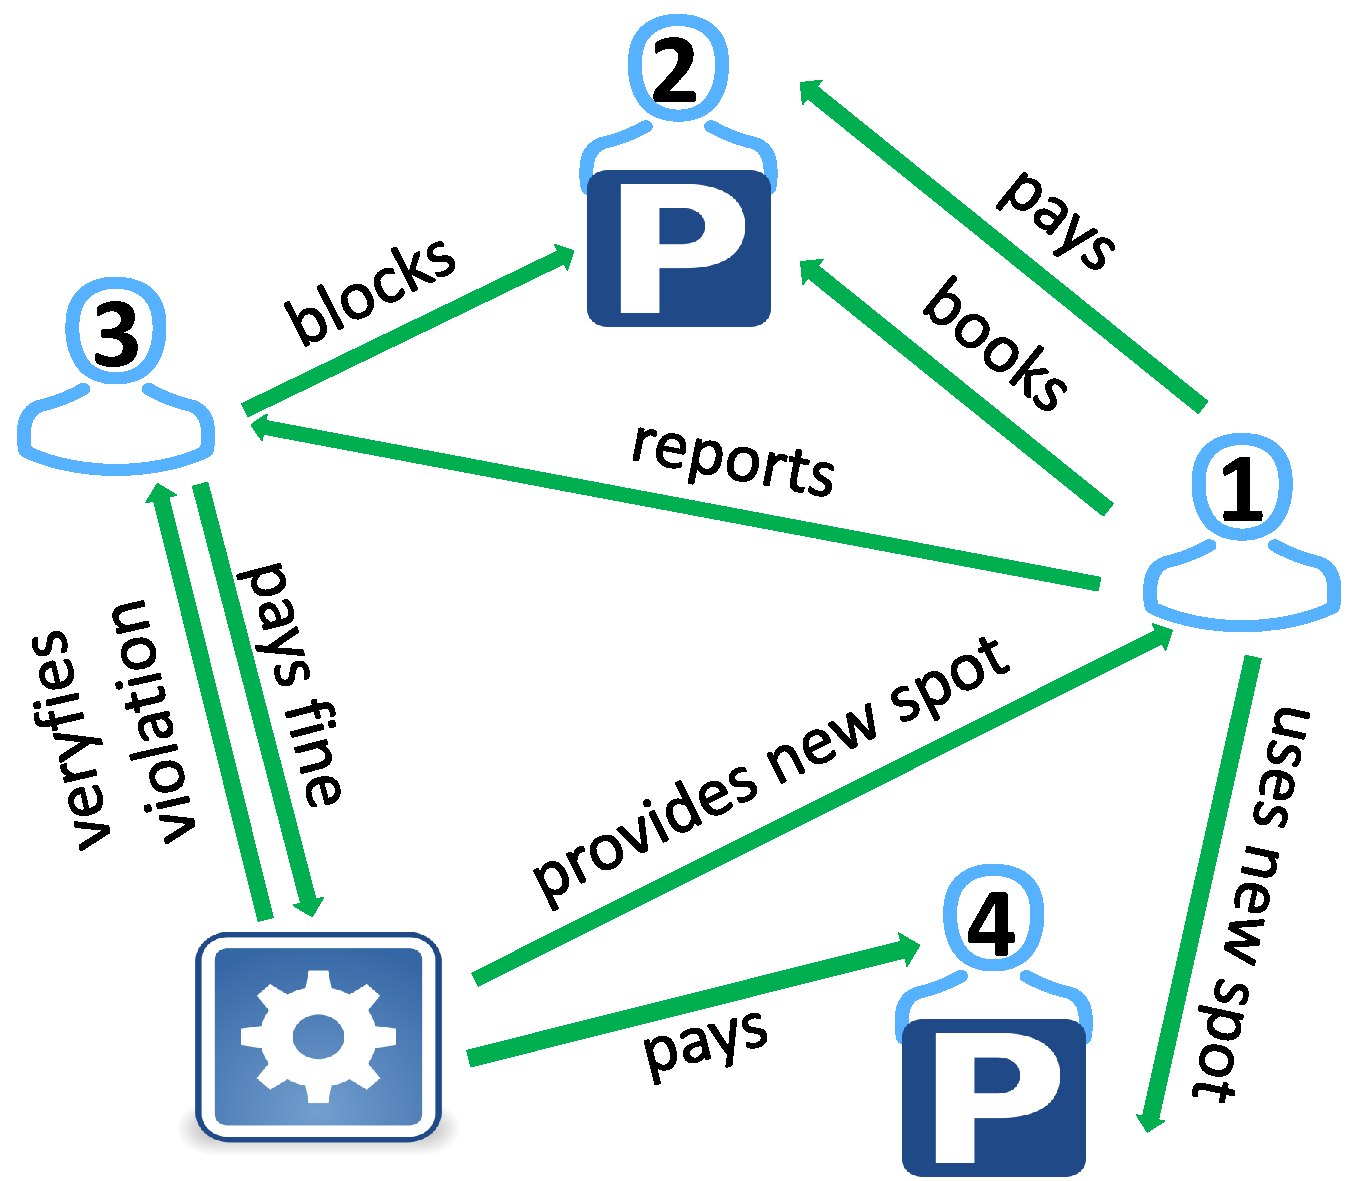
\includegraphics[width=13cm,height=11cm]{example_grafik.pdf}
	\caption{A possible example for the handling of fraud}
	\label{img:example-grafik}
\end{figure}
 
The case we have just discussed is clearly a class 1 fraud case, but it might also be as follows: $u_1$ arrives at the location of the booked parking space of $u_2$ and finds a free parking space. He, however, wants to harm $u_3$ and reports him nonetheless as a parking offender. This represents a corruption attack by $u_1$ and thus a fraud case of class 2. Like above the inspectors $u_{i1}$...$u_{i3}$ are requested, except this time they'll report that the parking lot is available. The reputation module evaluates all contributions and concludes that $u_1$ is the adversary. All reputation scores $R_{u_1}, R_{u_2}, R_{u_{i1}}, R_{u_{i2}}, R_{u_{i3}}$ are adjusted accordingly.\\

We can consider another variation of the first case presented. $u_3$, who has already been exposed as adversary several times, occupies the parking lot of $u_2$ without permission and is reported by $u_1$. After the inspector $u_{i1}$ has arrived and reported his contribution, $u_3$ leaves the parking space and the other two inspectors $u_{i2}$,$u_{i3}$ report that the parking space is free. The reputation module evaluates the contributions here as well. Only two of the five contributions ($C_{u_{1}}$ and $C_{u_{i1}}$) agree with the reporting user and therefore the truth, but the module would nevertheless count them as the truth expose $u_3$ as the adversary. This is because the trust of the two contributions $Trust(C_{u_{1}})$ and $Trust(C_{u_{i1}})$ that match the reporting user is significantly higher than the trust of the other three contributions $Trust(C_{u_{i2}})$,$Trust(C_{u_{i3}})$ and $Trust(C_{u_{3}})$. The reason for this is that the proximity factors $\sigma_{u_{i2}}$ and $\sigma_{u_{i3}}$ are lowered, because $u_{i2}$ and $u_{i3}$ arrived late at the location of the event and the reputation score $R_{u_3}$ is already low, because $u_3$ is a known adversary. Thus the module returns $u_3$ as the adversary.